\section{Introduction}
Humanoid robots have long been envisioned as general-purpose embodied intelligent agents capable of performing versatile tasks, that are anthromorphically compatible with our own actions. Recent progress has led to impressive demonstrations in locomotion~\cite{long2024learning} and motion imitation~\cite{liao2025beyond, xie2025kungfubot}. Nevertheless, most existing work remains focused on control in the free space or with static ground interaction. For example, maintaining balance~\cite{zhang2025hub}, walking~\cite{long2024learning}, or mimicking human poses~\cite{liao2025beyond}, while relatively few address the challenge of interacting with fast-moving objects in dynamic environments.


\begin{figure*}
    \centering
    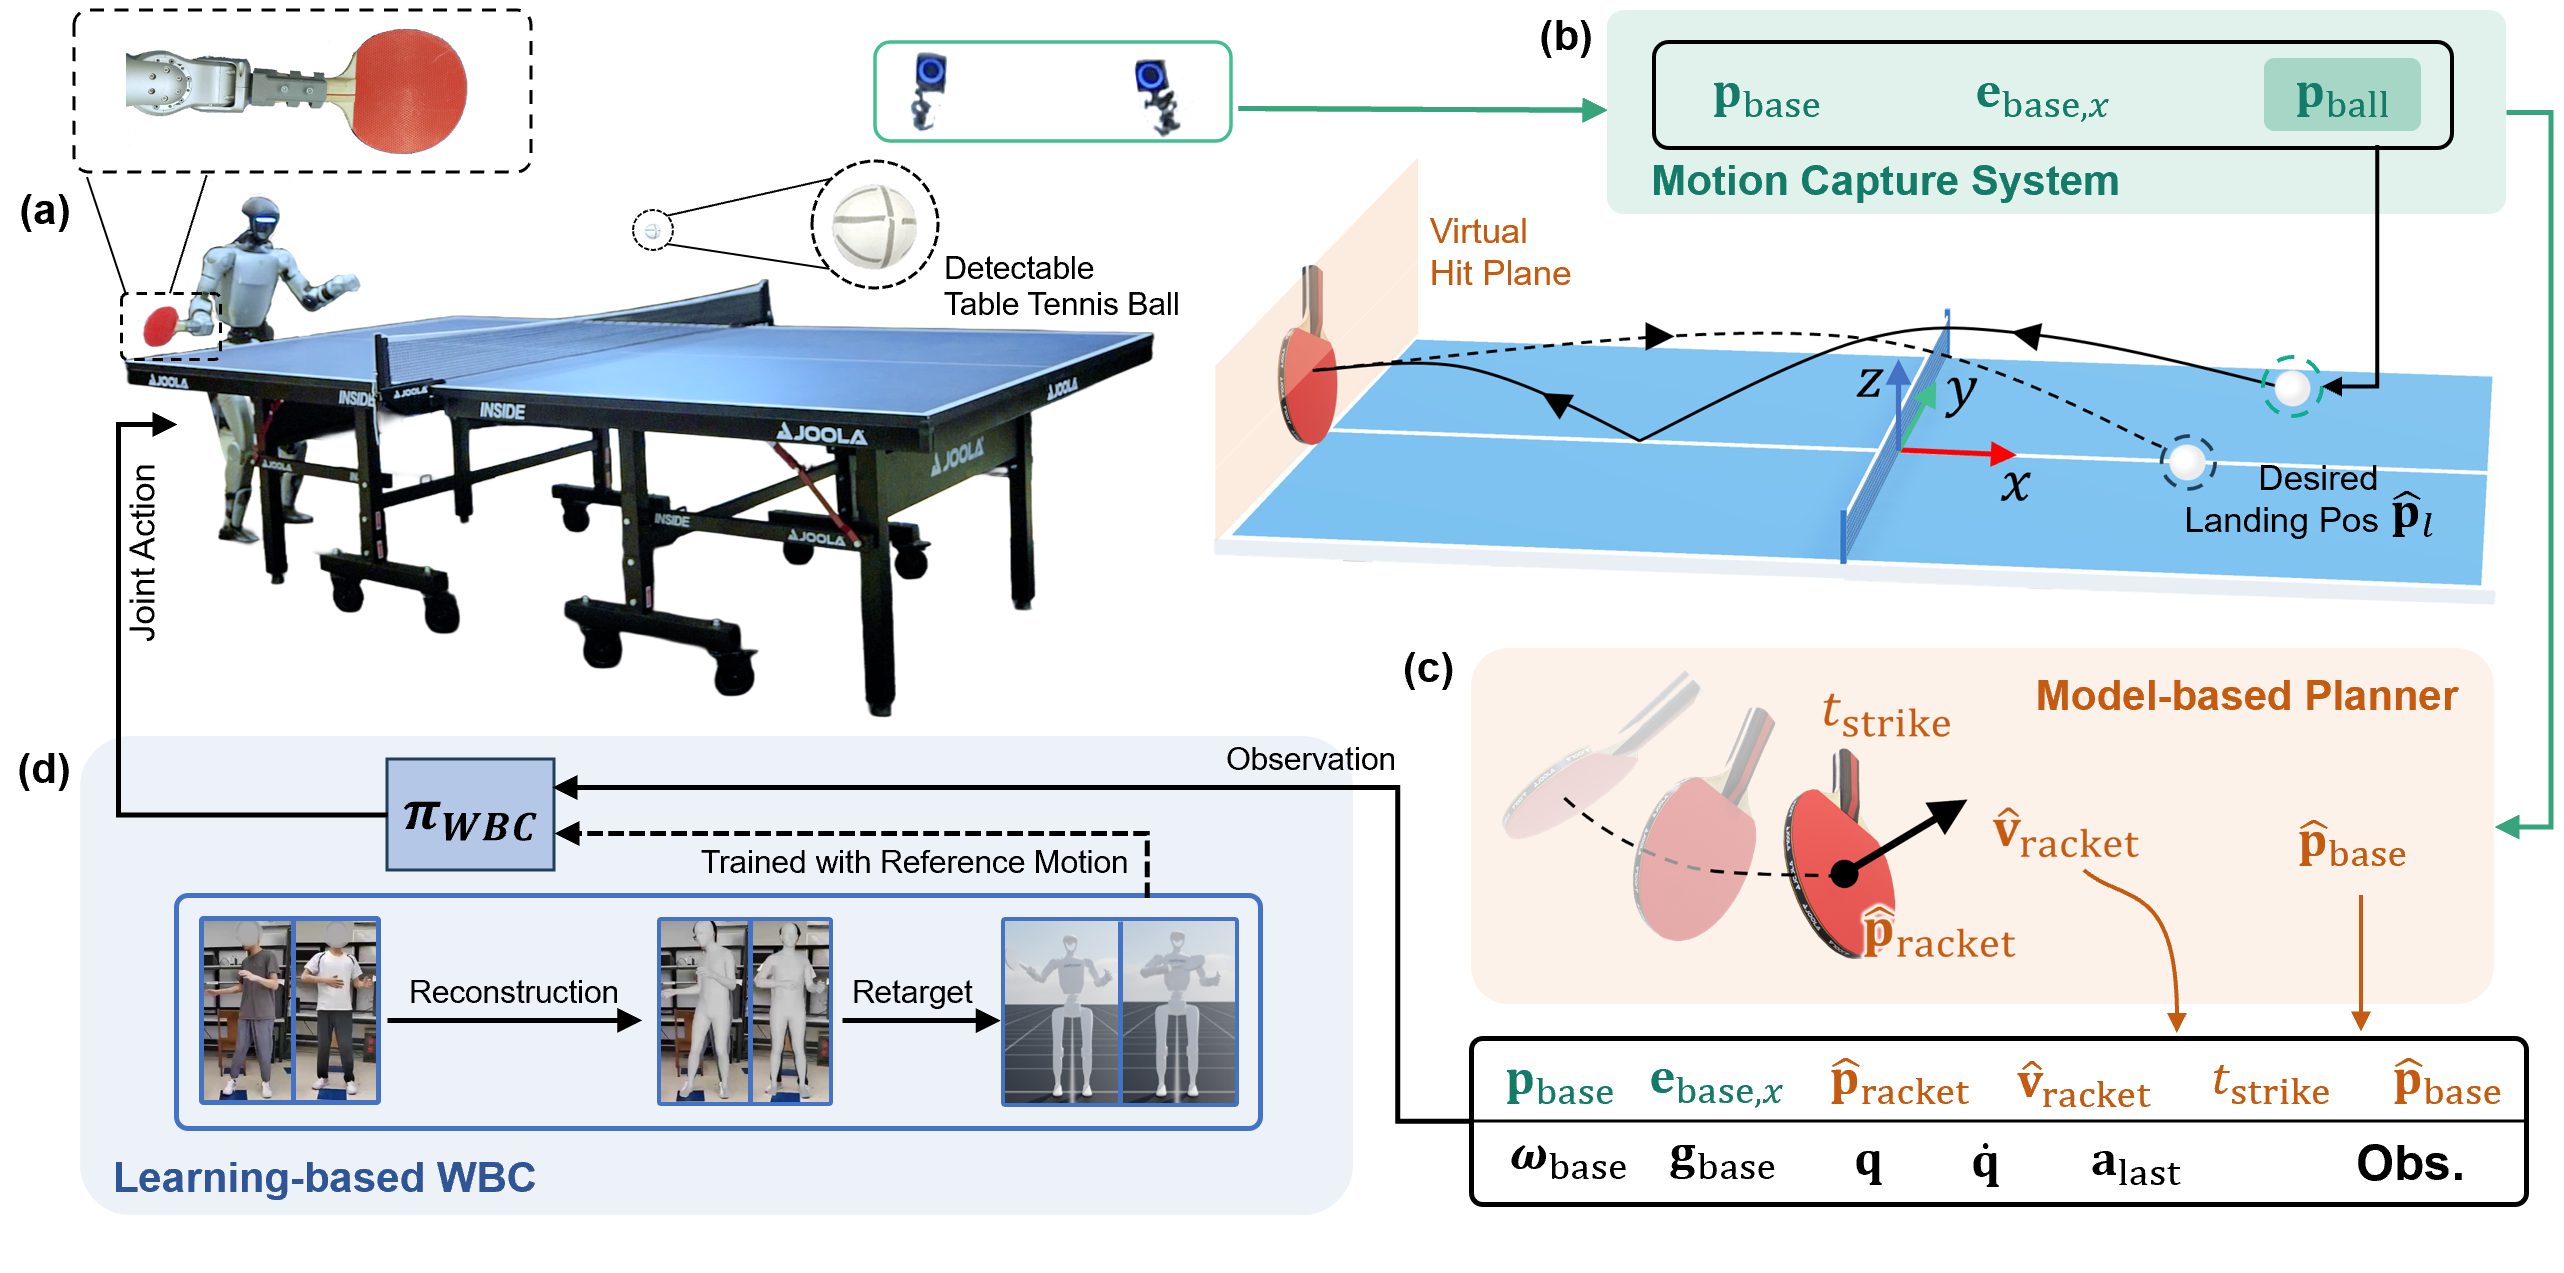
\includegraphics[width=\linewidth]{figures/framework.png}
    \caption{\textbf{System overview.} 
    (a) The racket is mounted on the robot’s right wrist using a 3D-printed connector, and the ball is covered with reflective tape for motion capture. 
    (b) The motion capture system tracks the ball position $\mathbf{p}_{\mathrm{ball}}$, the robot base position $\mathbf{p}_{\mathrm{base}}$, and the base forward vector $\mathbf{e}_{\mathrm{base},x}$. 
    (c) The model-based planner uses $\mathbf{p}_{\mathrm{ball}}$ and the desired landing point $\hat{\mathbf{p}}_l$ to predict the racket’s striking position $\hat{\mathbf{p}}_{\mathrm{racket}}$, velocity $\hat{\mathbf{v}}_{\mathrm{racket}}$, and strike time $t_{\mathrm{strike}}$. Given $\mathbf{p}_{\mathrm{base}}$ and $\hat{\mathbf{p}}_{\mathrm{racket}}$, the base target position $\hat{\mathbf{p}}_{\mathrm{base}}$ is also computed. 
    (d) The learning-based Whole Body Controller (WBC) policy $\pi_{WBC}$ is trained in simulation via reinforcement learning with human motion references and then deployed on the real robot. It takes as input the observations provided by other system components together with the robot’s proprioceptive information.}
    \label{fig:method}
\end{figure*}

Such interactions are fundamentally harder: they demand not only coordinated control across dozens of joints, but also tight perception-action loops operating at extreme time scales. Table tennis epitomizes this challenge. A ball traveling at over 5\,m/s allows for only sub-second reaction times, forcing the robot system to perceive, predict, plan, and strike within a few hundred milliseconds. Unlike locomotion or static manipulation, success requires agile whole-body movements, blending rapid arm swings with waist rotations, as well as quick stepping and balance recovery, to ensure accurate hit and readiness for the next rally. Compared to other racket sports, such as badminton~\cite{ma2025learning} or tennis~\cite{zaidi2023athletic}, table tennis poses an even greater challenge due to its shorter distances, faster exchanges, and smaller reaction windows. Humanoid table tennis therefore serves as a unique testbed for robotics because:
(a) it is highly dynamic, requiring fast ball trajectory prediction and strike planning;
(b) consecutive rallies necessitate agile motions and balance recovery after each stroke; and
(c) human-like striking motions are essential for both effectiveness and naturalness.

To address these challenges, we adopt a hierarchical framework that separates high-level planning from low-level control. At the high level, a model-based planner estimates the ball trajectory and predicts the striking position, velocity, and timing with high precision. At the low level, a reinforcement learning (RL)-based whole-body controller is trained to execute human-like striking motions while tracking the racket targets specified by the planner. This design directly addresses the identified challenges by: (a) having the planner provide fast trajectory prediction and strike planning, thereby offering a stable interface for the controller and improving sample efficiency during training; (b) training the RL controller on consecutive strikes so that it learns agile motions and reliable balance recovery; and (c) incorporating only two human reference motions into training, through which the controller acquires natural and human-like strikes.

Through extensive real-world experiments, including rallies against both humans and humanoids, we demonstrate that humanoid table tennis is feasible, marking a step toward agile and interactive humanoid behaviors. This is achieved using a general-purpose humanoid robot, without relying on specialized hardware. Notably, the system operates fully autonomously, without teleoperation. Our contributions are as follows:
\begin{itemize}
    \item We propose a hierarchical framework that integrates a model-based planner and an RL-based whole-body controller, enabling humanoid table tennis play.
    \item We develop human-like, whole-body striking skills, combining coordinated arm motions for multi-skill ball-hitting, and agile leg movements for rapid reaching.
    \item We validate our approach through extensive real-world experiments, including both humanoid-humanoid and humanoid-human rallies. Our humanoid achieves up to 106 consecutive shots against a human opponent.
\end{itemize}

